\documentclass[a4paper,12pt]{article}

%%% Alapdokumentum beállítások %%%
\usepackage[hungarian]{babel}     % Magyar nyelvi támogatás
\usepackage[T1]{fontenc}          % T1 betűtípus kódolás (az utf8 inputenc ma már alapértelmezett)
\usepackage{geometry}             % Oldalformázás
\geometry{a4paper, margin=1.5in}  % Papírméret és margók

%%% Szövegformázás és oldalelrendezés (JAVÍTOTT) %%%
\usepackage{microtype}            % Intelligens sorkizárás, szebb szövegkép
\usepackage{parskip}              % Bekezdések közötti térköz (behúzás helyett)
\usepackage{enumitem}             % Lista testreszabáshoz
\usepackage{multicol}             % Többszörös oszlopokhoz
\setlength{\emergencystretch}{3em}% Segít a nehezen törhető soroknál (a \sloppy helyett)
% Az elválasztás tiltása (\hyphenpenalty) kivezetve, mert magyar nyelvben tönkreteszi a sorkizárást!

%%% Matematikai és tudományos csomagok %%%
\usepackage{amsmath, amssymb, amsfonts, amsthm} % Matematikai csomagok egyben
\usepackage{stmaryrd}                           % Speciális matematikai szimbólumok
\usepackage[version=4]{mhchem}                  % Kémiai képletekhez
\usepackage{esvect}                             % Vektorokhoz (vastag nyilak)
\usepackage{cancel}                             % Matematikai áthúzáshoz

%%% Színek és Grafikai elemek (JAVÍTOTT) %%%
\usepackage{xcolor}                             % Színek kezelése (FONTOS!)
\definecolor{bvred}{rgb}{0.8, 0.0, 0.0}         % Piros szín definiálása
\definecolor{mainblue}{rgb}{0.1, 0.3, 0.6}      % Kék árnyalat a dobozokhoz
\definecolor{maingreen}{rgb}{0.1, 0.5, 0.2}     % Zöld árnyalat a dobozokhoz

\usepackage{graphicx}                           % Képek beszúrásához
\usepackage{wrapfig}                            % Képek lebegtetéséhez
\usepackage{tikz}                               % Vektoros ábrákhoz
\usetikzlibrary{calc, intersections, decorations.pathreplacing, arrows.meta}
\usepackage{pgfplots}
\pgfplotsset{compat=1.18}                       % PGFPlots kompatibilitás (FONTOS!)
\usepackage{caption}                            % Ábrafeliratok testreszabásához
\usepackage{float}                              % Ábrák pozicionálásához

%%% Táblázatok és tömbök %%%
\usepackage{array}                       % Speciális oszloptípusok
\setlength{\arrayrulewidth}{0.8pt}       % Táblázatvonalak vastagsága
\setlength{\tabcolsep}{6pt}              % Oszlopok közötti térköz
\renewcommand{\arraystretch}{1.8}        % Sorok magassága

%%% Egyedi parancsok és környezetek (JAVÍTOTT) %%%
\newcommand{\textbfr}[1]{\textbf{\textcolor{bvred}{#1}}} % Piros félkövér szöveg

\usepackage{etoolbox} % LaTeX programozási eszközök
\newrobustcmd*{\mytriangle}[1]{%                  % Háromszög jelölés
    \tikz{\filldraw[draw=#1,fill=#1,rotate=-90] (0,0)--(0.2cm,0)--(0.1cm,0.2cm)--cycle;}}

% amsthm környezetek letisztult beállítása
\theoremstyle{definition} % Ezzel a normál (nem dőlt) betűtípust használja a környezeteken belül
\newtheorem*{definition}{Definíció}
\newtheorem*{theorem}{Tétel}
\newtheorem*{problem}{Feladat}
\newtheorem*{example}{Példa}
\newtheorem*{remark}{\mytriangle{bvred} Megjegyzés}

%%% Hiperhivatkozások és PDF-beállítások %%%

%%% Megjelenítéshez automatikusan kiegészített csomagok %%%
\usepackage[utf8]{inputenc}
\usepackage{tcolorbox}
\tcbuselibrary{theorems,skins,breakable}
\usepackage{booktabs}

%%% Megjelenítéshez kiegészített dobozok és makrók %%%
\newtcolorbox{definiciodoboz}[1][]{colback=blue!5!white,colframe=mainblue,fonttitle=\bfseries,title=Definíció: #1}
\newtcolorbox{teteldoboz}[1][]{colback=green!8!white,colframe=maingreen,fonttitle=\bfseries,title=Tétel: #1}
\newtcolorbox{torvenydoboz}[1][]{colback=purple!5!white,colframe=purple!75!black,fonttitle=\bfseries,title=Fizikai törvény: #1}
\newtcolorbox{tippdoboz}[1][]{colback=yellow!10!white,colframe=orange!80!black,fonttitle=\bfseries,title=Megjegyzés: #1}

\usepackage{hyperref}                    % Mindig utolsóként (vagy majdnem utolsóként) érdemes betölteni

%%% Geometriai jelölések %%%
\def\dotMarkRightAngle[size=#1](#2,#3,#4){%
 \draw ($(#3)!#1!(#2)$) --
       ($($(#3)!#1!(#2)$)!#1!90:(#2)$) --
       ($(#3)!#1!(#4)$);
 \path (#3)--node[circle,fill,inner sep=.5pt]{} ($($(#3)!#1!(#2)$)!#1!90:(#2)$);
}

% TikZ alapstílusok
\tikzset{
    vertex/.style={circle, draw=black, fill=white, thick, minimum size=18pt, inner sep=0pt},
    oddvertex/.style={circle, draw=red, fill=red!15, very thick, minimum size=18pt, inner sep=0pt},
    edge/.style={thick, draw=black!70},
    highlightedge/.style={very thick, draw=red},
    patharrow/.style={-latex, thick, draw=blue!70!black} % Euler-vonal bejárásához
}


\title{Gráfok}
\author{AI LaTeX Studio}
\date{\today}

\begin{document}

\maketitle

\section{Bevezetés: Mik is azok a gráfok?}

A gráfelmélet a modern matematika és az informatika egyik legfontosabb területe. Gráfokkal modellezzük az internetes hálózatokat, az ismeretségi kapcsolatokat (közösségi média), az úthálózatokat és az elektromos áramköröket is.

Hadd nyugtassalak meg rögtön az elején: \textbf{a gráfok a matematika legszemléletesebb fejezetei közé tartoznak.}

A valóságban nem csinálunk mást, mint:
\begin{itemize}[leftmargin=2em]
    \item \textbf{objektumokat} (embereket, városokat, reptereket, weboldalakat) vizsgálunk – ezeket a matematikában \textbfr{csúcsoknak} (\textit{vertex}) nevezzük,
    \item és a köztük lévő \textbf{kapcsolatokat} (ismeretségeket, utakat, járatokat, linkeket) – ezek pedig az \textbfr{élek} (\textit{edge}).
\end{itemize}

\begin{definiciodoboz}[Gráf fogalma]
Egy $G = (V, E)$ \textbf{gráf} nem más, mint csúcsok egy nem üres $V$ halmaza, és a csúcspárokat összekötő $E$ élek halmaza.
\end{definiciodoboz}

Képzeld el, hogy négy barát – Anna ($A$), Béla ($B$), Cecília ($C$) és Dániel ($D$) – találkozik. Ha ketten ismerik egymást, összekötjük őket egy vonallal.

\begin{figure}[H]
    \centering
    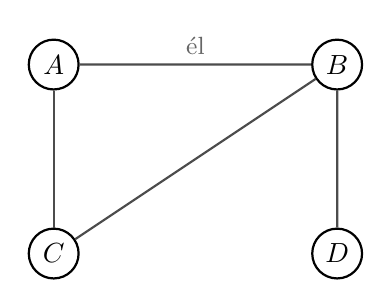
\begin{tikzpicture}[scale=1.2]
        \node[vertex] (A) at (0, 2) {$A$};
        \node[vertex] (B) at (3, 2) {$B$};
        \node[vertex] (C) at (0, 0) {$C$};
        \node[vertex] (D) at (3, 0) {$D$};

        \draw[edge] (A) -- (B) node[midway, above, font=\small, text=black!60] {él};
        \draw[edge] (A) -- (C);
        \draw[edge] (B) -- (C);
        \draw[edge] (B) -- (D);
    \end{tikzpicture}
    \caption{Egy egyszerű ismeretségi hálózat (4 csúcs, 4 él).}
    \label{fig:intro_graph}
\end{figure}

Látod? Ez az egész lényege. Semmi varázslat: az $A$, $B$, $C$, $D$ pontok a \textbf{csúcsok}, a vonalak pedig az \textbf{élek}.

---

\section{Alapfogalmak}

Nézzük át azokat a definíciókat, amelyeket a feladatok megoldásához kötelező magabiztosan ismerned! Minden fogalmat azonnal le is rajzolunk.

\subsection{A fokszám}

A fokszám az egyik leggyakoribb kulcsszó. Kérdezd meg magadtól: \textit{„Hány vonal indul ki ebből a pontból?”} Vagy a bulis példánál maradva: \textit{„Hány emberrel fogott kezet ez a vendég?”}

\begin{definiciodoboz}[Fokszám]
Egy csúcs \textbf{fokszáma} a csúcsba befutó (vagy abból kiinduló) élek száma. Jelölése: $d(v)$ (az angol \textit{degree} szóból).
\end{definiciodoboz}

\begin{figure}[H]
    \centering
    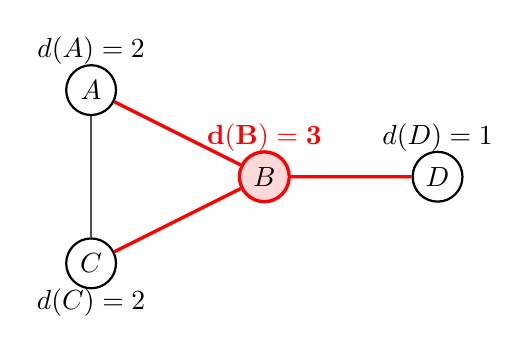
\begin{tikzpicture}[
        scale=1.1,
        vertex/.style={circle, draw=black, fill=white, thick, minimum size=18pt, inner sep=0pt},
        oddvertex/.style={circle, draw=red, fill=red!15, very thick, minimum size=18pt, inner sep=0pt},
        edge/.style={thick, draw=black!70},
        highlightedge/.style={very thick, draw=red}
    ]
        \node[vertex] (A) at (0,2) {$A$};
        \node[oddvertex] (B) at (2,1) {$B$};
        \node[vertex] (C) at (0,0) {$C$};
        \node[vertex] (D) at (4,1) {$D$};

        \draw[highlightedge] (B) -- (A);
        \draw[highlightedge] (B) -- (C);
        \draw[highlightedge] (B) -- (D);
        \draw[edge] (A) -- (C);

        \node[above=0.2cm] at (A) {$d(A) = 2$};
        \node[above=0.2cm, text=red] at (B) {$\mathbf{d(B) = 3}$};
        \node[below=0.2cm] at (C) {$d(C) = 2$};
        \node[above=0.2cm] at (D) {$d(D) = 1$};
    \end{tikzpicture}
    \caption{A $B$ csúcsból 3 él fut ki, így $d(B) = 3$. A többi csúcs fokszáma: $d(A)=2, d(C)=2, d(D)=1$.}
    \label{fig:degree}
\end{figure}

\subsection{Egyszerű gráf vs. "Nem egyszerű" elemek}

Középiskolában szinte mindig \textbf{egyszerű gráfokkal} dolgozunk. De mitől lesz egy gráf egyszerű? Attól, hogy nincsenek benne felesleges furcsaságok!
\begin{itemize}
    \item \textbf{Hurokél:} Olyan él, amely önmagába tér vissza (mintha valaki önmagával fogna kezet).
    \item \textbf{Többszörös (párhuzamos) él:} Két csúcs között több él is fut (kétszer fognak kezet).
\end{itemize}

\begin{definiciodoboz}[Egyszerű gráf]
Egy gráfot \textbf{egyszerűnek} nevezünk, ha nem tartalmaz sem hurokélt, sem párhuzamos éleket.
\end{definiciodoboz}

\begin{figure}[H]
    \centering
    \begin{tikzpicture}[scale=1.0]
        % Egyszerű gráf
        \begin{scope}[xshift=0cm]
            \node[vertex] (1) at (0,1.5) {$1$};
            \node[vertex] (2) at (2,1.5) {$2$};
            \node[vertex] (3) at (1,0) {$3$};
            \draw[edge] (1) -- (2);
            \draw[edge] (2) -- (3);
            \draw[edge] (3) -- (1);
            \node[below=0.3cm of 3] {\textbf{Egyszerű gráf}};
        \end{scope}

        % Nem egyszerű gráf
        \begin{scope}[xshift=6cm]
            \node[vertex] (u) at (0,1.5) {$u$};
            \node[vertex] (v) at (2,1.5) {$v$};

            % Többszörös él
            \draw[edge] (u) to[bend left=30] node[midway, above, font=\scriptsize, text=bvred] {többszörös él} (v);
            \draw[edge] (u) to[bend right=30] (v);

            % Hurokél
            \draw[edge] (u) to[out=135, in=225, looseness=8] node[left, font=\scriptsize, text=bvred] {hurokél} (u);

            \node at (1,-0.5) {\textbf{Nem egyszerű (multigráf)}};
        \end{scope}
    \end{tikzpicture}
    \caption{Egyszerű gráf és nem egyszerű gráf összehasonlítása.}
    \label{fig:simple_graph}
\end{figure}

\subsection{Út és Kör}

Hogyan tudunk sétálni a gráfban az élek mentén? Két nagyon fontos alapfogalmat kell megkülönböztetnünk:
\begin{itemize}
    \item \textbf{Út:} Egymáshoz csatlakozó élek olyan sorozata, ahol \textbfr{egyetlen csúcsot sem érintünk kétszer}. Olyan, mintha elindulnál a városban, és sosem térnél vissza olyan kereszteződésbe, ahol már jártál.
    \item \textbf{Kör:} Olyan zárt út, amely ugyanoda érkezik vissza, ahonnan elindult, de útközben nem érint kétszer semmilyen más csúcsot.
\end{itemize}

\begin{figure}[H]
    \centering
    \begin{tikzpicture}[scale=1.1]
        % Út ábra
        \begin{scope}[xshift=0cm]
            \node[vertex] (A) at (0,2) {$A$};
            \node[vertex] (B) at (2,2) {$B$};
            \node[vertex] (C) at (0,0) {$C$};
            \node[vertex] (D) at (2,0) {$D$};

            \draw[edge, dashed, black!30] (A) -- (B);
            \draw[edge, dashed, black!30] (B) -- (C);

            % Kiemelt út nyilakkal
            \draw[patharrow] (A) -- (C);
            \draw[patharrow] (C) -- (D);
            \draw[patharrow] (D) -- (B);

            \node[below=0.4cm of C, xshift=1cm] {\textbf{Út:} $A \to C \to D \to B$};
        \end{scope}

        % Kör ábra
        \begin{scope}[xshift=6cm]
            \node[vertex] (A) at (0,2) {$A$};
            \node[vertex] (B) at (2,2) {$B$};
            \node[vertex] (C) at (0,0) {$C$};
            \node[vertex] (D) at (2,0) {$D$};

            \draw[edge, dashed, black!30] (B) -- (D);

            % Kiemelt kör nyilakkal
            \draw[patharrow] (A) -- (B);
            \draw[patharrow] (B) -- (C);
            \draw[patharrow] (C) -- (A);

            \node[below=0.4cm of C, xshift=1cm] {\textbf{Kör:} $A \to B \to C \to A$};
        \end{scope}
    \end{tikzpicture}
    \caption{Út (nincs ismétlődő csúcs) és Kör (zárt útvonal) szemléltetése.}
    \label{fig:path_cycle}
\end{figure}

\subsection{Összefüggő gráfok}

Gondolj egy szigetekből és hidakból álló országra! El tudsz jutni száraz lábon bárhonnan bárhová?

\begin{definiciodoboz}[Összefüggő gráf]
Egy gráfot \textbf{összefüggőnek} nevezünk, ha bármely két csúcsa között vezet út (azaz a gráf \quotedblbase egy darabban van\textquotedblleft). Ha a gráf különálló darabokra esik szét, akkor \textbf{nem összefüggő}, és a darabjait \textbf{komponenseknek} hívjuk.
\end{definiciodoboz}

\begin{figure}[H]
    \centering
    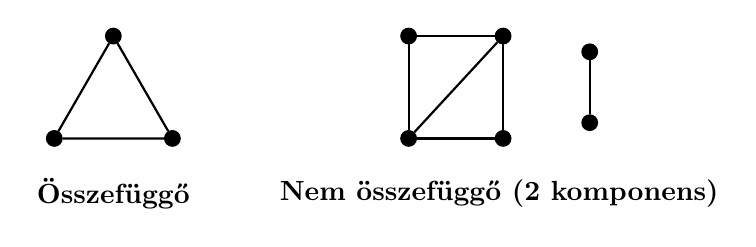
\begin{tikzpicture}[
        scale=1.0,
        vertex/.style={circle, draw=black, fill=black, inner sep=2pt},
        edge/.style={thick}
    ]
        % Összefüggő
        \begin{scope}[xshift=0cm]
            \node[vertex] (1) at (0,0) {};
            \node[vertex] (2) at (1.5,0) {};
            \node[vertex] (3) at (0.75,1.3) {};
            \draw[edge] (1) -- (2) -- (3) -- (1);
            \node at (0.75, -0.7) {\textbf{Összefüggő}};
        \end{scope}

        % Nem összefüggő
        \begin{scope}[xshift=4.5cm]
            % 1. komponens (4 csúcsú részgráf)
            \node[vertex] (A) at (0,0) {};
            \node[vertex] (B) at (1.2,0) {};
            \node[vertex] (C) at (1.2,1.3) {};
            \node[vertex] (D) at (0,1.3) {};
            \draw[edge] (A) -- (B) -- (C) -- (D) -- (A);
            \draw[edge] (A) -- (C);

            % 2. komponens (kisebb, 2 csúcsú komponens)
            \node[vertex] (E) at (2.3,0.2) {};
            \node[vertex] (F) at (2.3,1.1) {};
            \draw[edge] (E) -- (F);

            \node at (1.15, -0.7) {\textbf{Nem összefüggő (2 komponens)}};
        \end{scope}
    \end{tikzpicture}
    \caption{Összefüggő gráf és több komponensből álló gráf.}
    \label{fig:connected}
\end{figure}

\subsection{Gráfok összehasonlítása: Izomorfia}

Gyakran találkozhatsz azzal a problémával, hogy két gráfot ránézésre különbözőnek ítélsz, de valójában pontosan ugyanazok, csak másképp vannak felrajzolva vagy a csúcsaik más címkével vannak ellátva. Ezt a tulajdonságot nevezzük izomorfiának.

\begin{definiciodoboz}[Izomorf gráfok]
Két gráf, $G_1 = (V_1, E_1)$ és $G_2 = (V_2, E_2)$ \textbf{izomorf}, ha létezik egy $f: V_1 \to V_2$ bijektív (egy-egy és szürjektív) leképezés, amely megtartja az élek struktúráját. Ez azt jelenti, hogy:
\begin{enumerate}
    \item $u,v \in V_1$ akkor és csak akkor van éllel összekötve $G_1$-ben, ha $f(u), f(v) \in V_2$ éllel össze van kötve $G_2$-ben.
    \item Az élek száma megegyezik: $|E_1| = |E_2|$.
    \item A csúcsok száma megegyezik: $|V_1| = |V_2|$.
    \item A fokszámok is azonosak (az $f$ leképezés szerint).
\end{enumerate}
Egyszerűen fogalmazva, az izomorf gráfok \textbfr{ugyanazt a struktúrát} mutatják, csak a csúcsok azonosítóit (címkéit) vagy a rajz elrendezését változtattuk meg.
\end{definiciodoboz}

\begin{figure}[H]
    \centering
    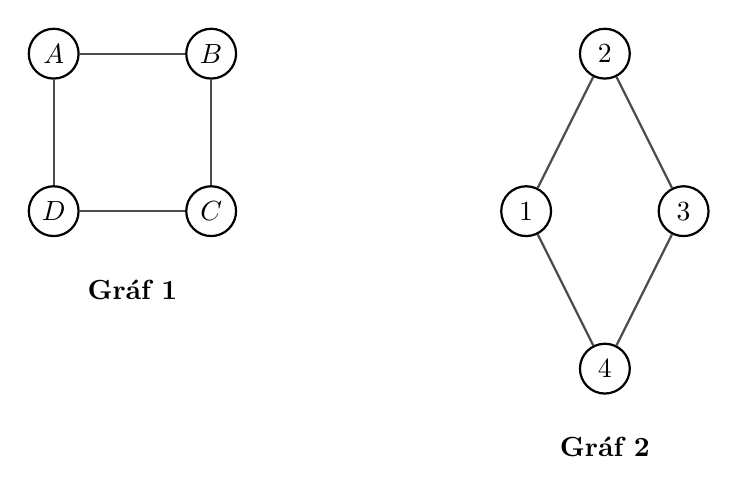
\begin{tikzpicture}[scale=1.0]
        % Első gráf
        \begin{scope}[xshift=0cm]
            \node[vertex] (A) at (0,2) {$A$};
            \node[vertex] (B) at (2,2) {$B$};
            \node[vertex] (C) at (2,0) {$C$};
            \node[vertex] (D) at (0,0) {$D$};
            \draw[edge] (A) -- (B) -- (C) -- (D) -- (A);
            \node at (1, -1) {\textbf{Gráf 1}};
        \end{scope}

        % Második gráf (izomorf az elsővel)
        \begin{scope}[xshift=6cm]
            \node[vertex] (1) at (0,0) {$1$};
            \node[vertex] (2) at (1,2) {$2$};
            \node[vertex] (3) at (2,0) {$3$};
            \node[vertex] (4) at (1,-2) {$4$};
            \draw[edge] (1) -- (2) -- (3) -- (4) -- (1);
            \node at (1, -3) {\textbf{Gráf 2}};
        \end{scope}
    \end{tikzpicture}
    \caption{Két izomorf gráf: mindkettő egy 4 csúcsú körgráf ($C_4$). Bár másképp vannak elrendezve és más csúcsneveket használnak, a belső struktúrájuk azonos.}
    \label{fig:isomorphic_graphs}
\end{figure}

---

\section{Általános képletek: A Kézfogási Lemma}

Most érkeztünk el a gráfok legfontosabb alaptételéhez. Ezt a feladatok felében használnod kell, úgyhogy alaposan értsük meg a logikáját!

\begin{teteldoboz}[A fokszámok összege / Kézfogási lemma]
Bármely egyszerű gráfban a csúcsok fokszámainak összege megegyezik az élek számának kétszeresével:
\begin{equation}
    \sum_{v \in V} d(v) = d(v_1) + d(v_2) + \dots + d(v_n) = 2 \cdot |E|
\end{equation}
ahol $|E|$ a gráf éleinek számát jelöli.
\end{teteldoboz}

\textbf{Miért van ez így?}\\
Gondolj egy kézfogásra! Ahhoz, hogy egy kézfogás (egy él) létrejöjjön, pontosan \textbf{két} ember nyújtja a kezét. Amikor a buli végén megkérdezzük az összes vendéget, hogy hányszor fogott kezet (összeadjuk a fokszámokat), minden egyes kézfogást pontosan kétszer számoltunk meg: egyszer az egyik, egyszer a másik félnél!

\begin{tippdoboz}[Az életmentő következmény!]
Mivel a fokszámok összege $2 \cdot |E|$, ami egy páros szám, ebből egyenesen következik:
\begin{center}
    \textbfr{Minden gráfban a páratlan fokszámú csúcsok száma PÁROS!}
\end{center}
Ha egy dolgozatban azt kérdezik: \textit{„Létezhet-e olyan társaság, ahol 5 embernek egyaránt 3 ismerőse van?”}, azonnal rávághatod: \textbf{NEM}, mert ekkor a páratlan fokszámú csúcsok száma 5 lenne (ami páratlan), vagy a fokszámok összege $5 \times 3 = 15$ lenne, ami nem lehet egy egész szám kétszerese!
\end{tippdoboz}

---

\section{Speciális gráfok}

Az érettségin kiemelten szeretnek két speciális gráftípust számonkérni. Nézzük meg ezeket részletesen!

\subsection{1. A teljes gráf ($K_n$)}

Képzeld el, hogy a társaságban \textbf{mindenki ismer mindenkit}, vagy egy sakkbajnokságon mindenki játszik mindenkivel pontosan egy meccset. Ezt hívjuk teljes gráfnak.

\begin{definiciodoboz}[Teljes gráf]
Az $n$ csúcsú \textbf{teljes gráfot} $K_n$-nel jelöljük. Ebben minden lehetséges él be van húzva, azaz bármely két különböző csúcs össze van kötve éllel.
\end{definiciodoboz}

\textbf{Mennyi éle van egy $K_n$ gráfnak?}
Kétféleképpen is könnyedén kiszámolhatod:
\begin{enumerate}
    \item Minden csúcs a nála lévő összes többi ($n-1$) csúccsal össze van kötve, így minden csúcs fokszáma $n-1$. A Kézfogási Lemma miatt:
    \[
    2 \cdot |E| = n \cdot (n-1) \implies |E| = \frac{n(n-1)}{2}
    \]
    \item Kombinatorikusan: $n$ emberből kell kiválasztanunk 2 embert, akik kezet fognak. A lehetőségek száma: $\binom{n}{2} = \frac{n(n-1)}{2}$.
\end{enumerate}

\begin{figure}[H]
    \centering
    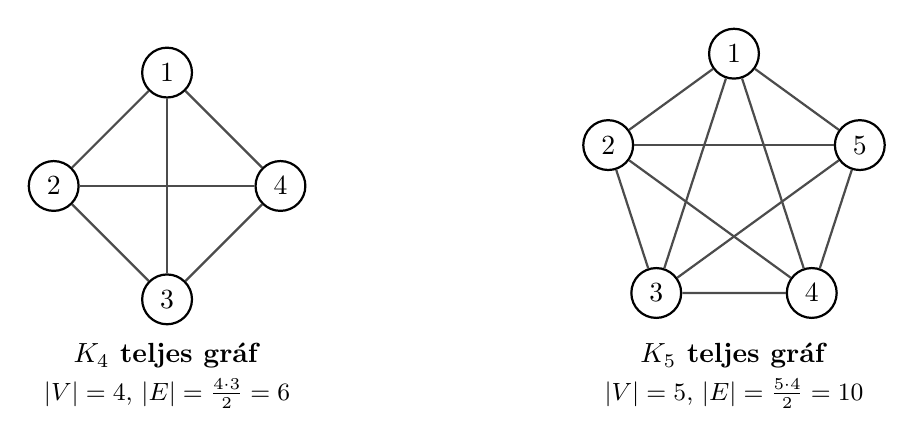
\begin{tikzpicture}[scale=1.2]
        % K4
        \begin{scope}[xshift=0cm]
            \foreach \i in {1,...,4} {
                \node[vertex] (v\i) at ({90 + (\i-1)*90}:1.2) {\i};
            }
            \foreach \i in {1,...,4} {
                \foreach \j in {\i,...,4} {
                    \ifnum\i<\j
                        \draw[edge] (v\i) -- (v\j);
                    \fi
                }
            }
            \node at (0, -1.8) {\textbf{$K_4$ teljes gráf}};
            \node at (0, -2.2) {\small $|V|=4$, $|E| = \frac{4 \cdot 3}{2} = 6$};
        \end{scope}

        % K5
        \begin{scope}[xshift=6cm]
            \foreach \i in {1,...,5} {
                \node[vertex] (w\i) at ({90 + (\i-1)*72}:1.4) {\i};
            }
            \foreach \i in {1,...,5} {
                \foreach \j in {\i,...,5} {
                    \ifnum\i<\j
                        \draw[edge] (w\i) -- (w\j);
                    \fi
                }
            }
            \node at (0, -1.8) {\textbf{$K_5$ teljes gráf}};
            \node at (0, -2.2) {\small $|V|=5$, $|E| = \frac{5 \cdot 4}{2} = 10$};
        \end{scope}
    \end{tikzpicture}
    \caption{A $K_4$ és $K_5$ teljes gráfok.}
    \label{fig:complete_graphs}
\end{figure}

\subsection{2. A fa gráf (Fák és erdők)}

A fa a természetben sem tartalmaz zárt hurkokat vagy köröket: az ágak csak szétágaznak. A matematikában is pontosan ezt jelenti!

\begin{definiciodoboz}[Fa gráf]
Egy gráfot \textbf{fának} nevezünk, ha \textbf{összefüggő} és \textbf{körmentes}.
\end{definiciodoboz}

\begin{figure}[H]
    \centering
    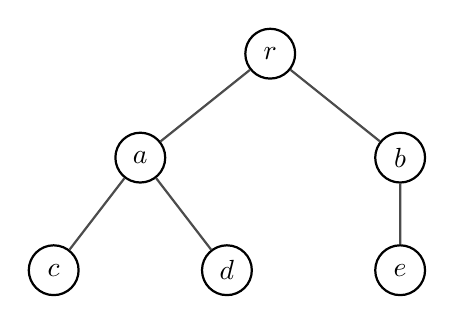
\begin{tikzpicture}[scale=1.1]
        \node[vertex] (r) at (3, 2.5) {$r$};
        \node[vertex] (a) at (1.5, 1.3) {$a$};
        \node[vertex] (b) at (4.5, 1.3) {$b$};
        \node[vertex] (c) at (0.5, 0) {$c$};
        \node[vertex] (d) at (2.5, 0) {$d$};
        \node[vertex] (e) at (4.5, 0) {$e$};

        \draw[edge] (r) -- (a);
        \draw[edge] (r) -- (b);
        \draw[edge] (a) -- (c);
        \draw[edge] (a) -- (d);
        \draw[edge] (b) -- (e);
    \end{tikzpicture}
    \caption{Egy 6 csúcsú fa gráf. Nincsen benne semmilyen kör, és egyetlen darabból áll.}
    \label{fig:tree_graph}
\end{figure}

\begin{teteldoboz}[A fa éleinek száma]
Minden $n$ csúcsú fára kivétel nélkül érvényes, hogy az éleinek száma pontosan eggyel kevesebb a csúcsok számánál:
\begin{equation}
    |E| = n - 1
\end{equation}
\end{teteldoboz}

Nézd meg a fenti ábrát: 6 csúcs van ($r, a, b, c, d, e$), az élek száma pedig pontosan $6 - 1 = 5$. Ha behúznál még egyetlen élt bárhová (pl. $c$ és $d$ közé), azonnal létrejönne egy kör, és máris elveszítené fa tulajdonságát!

\subsection{3. Komplementer gráf}

A komplementer gráf egy eredeti gráfból képzett új gráf, amely pontosan azokat az éleket tartalmazza, amelyek az eredeti gráfban hiányoznak, ha a teljes gráfot vesszük alapul.

\begin{definiciodoboz}[Komplementer gráf]
Adott egy $G = (V, E)$ egyszerű gráf. Ennek \textbf{komplementere} (jelölése: $\bar{G}$ vagy $G^c$) az a gráf, amelynek ugyanaz a csúcshalmaza $V$, mint $G$-nek, de két csúcs között akkor van él $\bar{G}$-ben, ha $G$-ben \textbf{nincs} közöttük él. Fordítva: ha $G$-ben van él közöttük, akkor $\bar{G}$-ben nincs.
\end{definiciodoboz}

\textbf{Példa:} Tekintsünk egy 4 csúcsú $G$ gráfot, amelynek csak két éle van.
\begin{figure}[H]
    \centering
    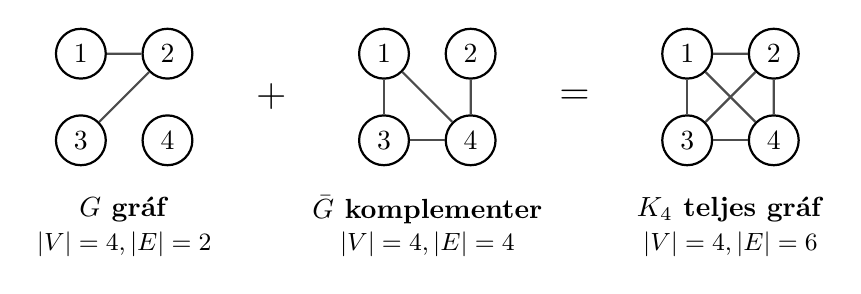
\begin{tikzpicture}[scale=1.1]
        % Gráf G
        \begin{scope}[xshift=0cm]
            \node[vertex] (1) at (0,1) {$1$};
            \node[vertex] (2) at (1,1) {$2$};
            \node[vertex] (3) at (0,0) {$3$};
            \node[vertex] (4) at (1,0) {$4$};

            \draw[edge] (1) -- (2);
            \draw[edge] (2) -- (3);

            \node at (0.5, -0.8) {\textbf{$G$ gráf}};
            \node at (0.5, -1.2) {\small $|V|=4, |E|=2$};
        \end{scope}

        % Plusz jel
        \node at (2.2, 0.5) {\Large $+$};

        % Gráf G komplementere
        \begin{scope}[xshift=3.5cm]
            \node[vertex] (1) at (0,1) {$1$};
            \node[vertex] (2) at (1,1) {$2$};
            \node[vertex] (3) at (0,0) {$3$};
            \node[vertex] (4) at (1,0) {$4$};

            % Élek, amik hiányoztak G-ben
            \draw[edge] (1) -- (3);
            \draw[edge] (1) -- (4);
            \draw[edge] (2) -- (4);
            \draw[edge] (3) -- (4);

            \node at (0.5, -0.8) {\textbf{$\bar{G}$ komplementer}};
            \node at (0.5, -1.2) {\small $|V|=4, |E|=4$};
        \end{scope}

        % Egyenlőségjel
        \node at (5.7, 0.5) {\Large $=$};

        % Teljes gráf (összeg/unió)
        \begin{scope}[xshift=7cm]
            \node[vertex] (1) at (0,1) {$1$};
            \node[vertex] (2) at (1,1) {$2$};
            \node[vertex] (3) at (0,0) {$3$};
            \node[vertex] (4) at (1,0) {$4$};

            % Összes él (G élei + komplementer élei)
            \draw[edge] (1) -- (2);
            \draw[edge] (2) -- (3);
            \draw[edge] (1) -- (3);
            \draw[edge] (1) -- (4);
            \draw[edge] (2) -- (4);
            \draw[edge] (3) -- (4);

            \node at (0.5, -0.8) {\textbf{$K_4$ teljes gráf}};
            \node at (0.5, -1.2) {\small $|V|=4, |E|=6$};
        \end{scope}
    \end{tikzpicture}
    \caption{A $G$ gráf és $\bar{G}$ komplementere, valamint összeadásuk (uniójuk), amely a $K_4$ teljes gráfot eredményezi. Figyeld meg, hogy az élek száma összeadódva pontosan a teljes gráf éleinek számát adja: $2 + 4 = 6 = \frac{4 \cdot 3}{2}$.}
    \label{fig:complement_graph}
\end{figure}

---

\section{Az Euler-vonal: Megrajzolható-e egyetlen vonallal?}

Biztosan te is játszottál gyerekkorodban azzal, hogy megpróbáltad lerajzolni a klasszikus „nyitott borítékot” úgy, hogy nem emeled fel a ceruzádat a papírról, és egyetlen vonalon sem mész át kétszer. Ez a híres **Euler-vonal** problémája!

\begin{definiciodoboz}[Euler-vonal]
Egy gráfban az \textbf{Euler-vonal} olyan élsorozat, amely a gráf \textbfr{minden élét pontosan egyszer} tartalmazza.
\begin{itemize}
    \item \textbf{Zárt Euler-vonal (Euler-kör):} Ugyanabba a csúcsba tér vissza, ahonnan elindult.
    \item \textbf{Nyílt Euler-vonal:} Különböző csúcsban ér véget, mint ahonnan indult.
\end{itemize}
\end{definiciodoboz}

\begin{teteldoboz}[Euler tétele a rajzolhatóságról]
Egy összefüggő gráfban akkor és csak akkor létezik:
\begin{enumerate}
    \item \textbf{Zárt Euler-vonal}, ha \textbfr{minden csúcs fokszáma páros}.
    \item \textbf{Nyílt Euler-vonal}, ha \textbfr{pontosan 2 darab páratlan fokszámú csúcs} van a gráfban (a többi csúcs páros). Ekkor a rajzolást kötelező az egyik páratlan csúcsból indítani, és a másik páratlan csúcsban fogjuk befejezni!
\end{enumerate}
\end{teteldoboz}

\begin{figure}[H]
    \centering
    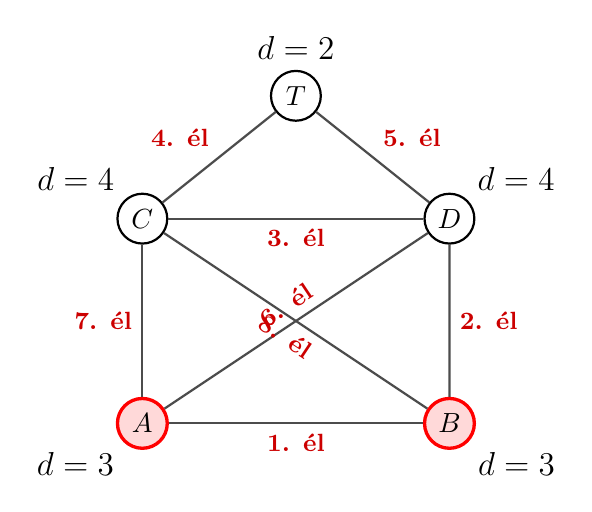
\begin{tikzpicture}[scale=1.3]
        % A házikó csúcsai
        \node[oddvertex, label=below left:{\large $d=3$}] (A) at (0,0) {$A$};
        \node[oddvertex, label=below right:{\large $d=3$}] (B) at (3,0) {$B$};
        \node[vertex, label=above left:{\large $d=4$}] (C) at (0,2) {$C$};
        \node[vertex, label=above right:{\large $d=4$}] (D) at (3,2) {$D$};
        \node[vertex, label=above:{\large $d=2$}] (T) at (1.5,3.2) {$T$};

        % Élek számozással ellátva a bejáráshoz
        \draw[edge] (A) -- (B) node[midway, below, font=\bfseries\small, text=bvred] {1. él};
        \draw[edge] (B) -- (D) node[midway, right, font=\bfseries\small, text=bvred] {2. él};
        \draw[edge] (D) -- (C) node[midway, below, font=\bfseries\small, text=bvred] {3. él};
        \draw[edge] (C) -- (T) node[midway, above left, font=\bfseries\small, text=bvred] {4. él};
        \draw[edge] (T) -- (D) node[midway, above right, font=\bfseries\small, text=bvred] {5. él};
        \draw[edge] (D) -- (A) node[midway, above, sloped, font=\bfseries\small, text=bvred] {6. él};
        \draw[edge] (A) -- (C) node[midway, left, font=\bfseries\small, text=bvred] {7. él};
        \draw[edge] (C) -- (B) node[midway, below, sloped, font=\bfseries\small, text=bvred] {8. él};
    \end{tikzpicture}
    \caption{A klasszikus „boríték-házikó”: $d(A)=3, d(B)=3$ páratlanok (pirossal jelölve), míg $d(C)=4, d(D)=4, d(T)=2$ párosak. Mivel pontosan 2 páratlan csúcs van, a gráf egy vonallal megrajzolható: $A$-ból indulunk, és $B$-ben végzünk!}
    \label{fig:envelope}
\end{figure}

---

\section{Típusfeladatok}

Nézzünk most három klasszikus feladattípust, amivel szinte biztosan találkozni fogsz a vizsgán!

\begin{problem}
Létezik-e olyan 5 csúcsú egyszerű gráf, amelynek fokszámai a következők:
\begin{enumerate}[label=(\alph*)]
    \item $1, 2, 2, 3, 3$
    \item $1, 3, 3, 3, 4$
    \item $2, 2, 2, 2, 2$
\end{enumerate}
\end{problem}

\begin{example}[\textbf{Megoldás lépésről lépésre}]
Mindig ezzel a két gyors szűrővel kezdj:
\begin{enumerate}
    \item \textbf{1. szűrő (Kézfogási lemma):} Add össze a fokszámokat! Ha a kapott összeg páratlan, a válasz \textbf{azonnal NEM}.
    \item \textbf{2. szűrő (Maximum fokszám):} Egy $n$ csúcsú egyszerű gráfban a maximális fokszám legfeljebb $n-1$ lehet (senki sem foghat kezet önmagával).
\end{enumerate}

Nézzük az eseteket:
\begin{itemize}[leftmargin=2em]
    \item[(a)] Összeg: $1 + 2 + 2 + 3 + 3 = 11$. \textbfr{Páratlan!} Nem létezhet, mert a páratlan fokszámú csúcsok száma 3 lenne (páratlan).
    \item[(b)] Összeg: $1 + 3 + 3 + 3 + 4 = 14$ (páros). Páratlan csúcsok száma: 4 darab (szintén páros). Elsőre jónak tűnik! De nézzük meg alaposabban:
    Van egy 4-es fokszámú csúcs ($v_5$). Mivel egyszerű gráfról van szó, ez az ember \textbf{mindenki mással} kezet fogott! Tehát minden más csúcsnak legalább 1-nek kell lennie a fokszámának. Ez teljesül.
    Próbáljuk meg felrajzolni a lehetséges gráfot!
\end{itemize}

\begin{figure}[H]
    \centering
    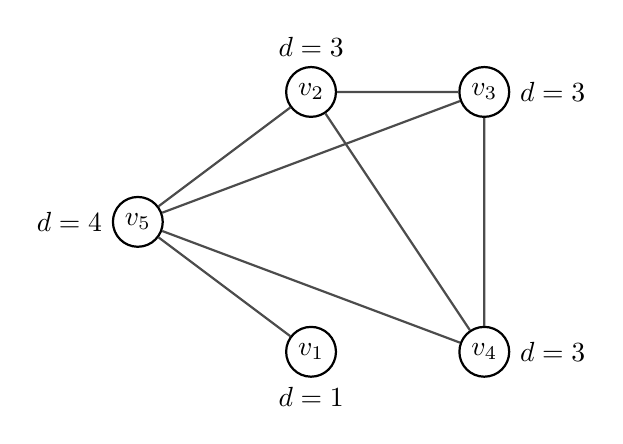
\begin{tikzpicture}[scale=1.1]
        \node[vertex, label=left:{$d=4$}] (E) at (0, 1.5) {$v_5$};
        \node[vertex, label=above:{$d=3$}] (A) at (2, 3) {$v_2$};
        \node[vertex, label=right:{$d=3$}] (B) at (4, 3) {$v_3$};
        \node[vertex, label=right:{$d=3$}] (C) at (4, 0) {$v_4$};
        \node[vertex, label=below:{$d=1$}] (D) at (2, 0) {$v_1$};

        % v5 összekötve mindenkivel
        \draw[edge] (E) -- (A);
        \draw[edge] (E) -- (B);
        \draw[edge] (E) -- (C);
        \draw[edge] (E) -- (D);

        % További élek v2, v3, v4 között, hogy fokszámuk 3 legyen
        \draw[edge] (A) -- (B);
        \draw[edge] (B) -- (C);
        \draw[edge] (A) -- (C);
    \end{tikzpicture}
    \caption{A (b) feladathoz tartozó megvalósítható egyszerű gráf: $d(v_1)=1, d(v_2)=3, d(v_3)=3, d(v_4)=3, d(v_5)=4$.}
    \label{fig:solution_b}
\end{figure}

Látható, hogy az ábrán $v_1$ foka 1, $v_5$ foka 4, a többiek foka pedig pontosan 3. Tehát \textbf{létezik ilyen gráf}!

\begin{itemize}[leftmargin=2em]
    \item[(c)] Fokszámok: $2, 2, 2, 2, 2$. Összeg: $2 \cdot 5 = 10$ (páros). Minden csúcs foka 2. Ez nem más, mint egy 5 hosszúságú kör ($C_5$)!
\end{itemize}

\begin{figure}[H]
    \centering
    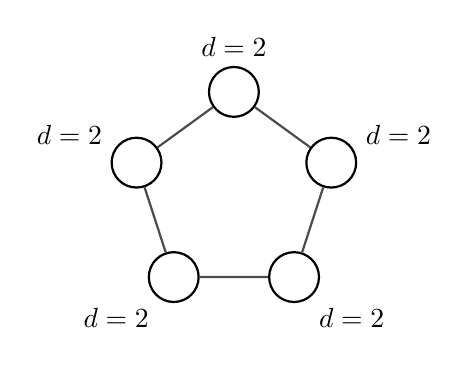
\begin{tikzpicture}[scale=1.0]
        \foreach \i in {1,...,5} {
            \node[vertex, label={{90 + (\i-1)*72}:{$d=2$}}] (c\i) at ({90 + (\i-1)*72}:1.3) {};
        }
        \draw[edge] (c1) -- (c2) -- (c3) -- (c4) -- (c5) -- (c1);
    \end{tikzpicture}
    \caption{Az 5 csúcsú, 2-reguláris körgráf ($C_5$). Minden fokszám pontosan 2.}
    \label{fig:c5_graph}
\end{figure}
\end{example}

---

\begin{problem}[Életszerű példa: A parkolóőr útvonala]
Egy pláza őre éjszaka szeretné ellenőrizni a mélygarázs összes útszakaszát. Az utak elrendezését az alábbi alaprajz mutatja. Végig tud-e menni az összes útszakaszon úgy, hogy \textbf{minden szakaszon pontosan egyszer halad végig}, és nem kell egyetlen útra sem visszatérnie? Ha igen, honnan kell indulnia?
\end{problem}

\begin{example}[\textbf{Megoldás}]
\textbf{1. Lépés:} Fordítsuk le a feladatot a matematika nyelvére!
Az útszakaszok az élek, a kereszteződések a csúcsok. A feladat szövege azt kéri, hogy minden élen pontosan egyszer menjünk végig $\implies$ \textbf{Euler-vonalat keresünk!}

\textbf{2. Lépés:} Határozzuk meg az összes csúcs fokszámát!

\begin{figure}[H]
    \centering
    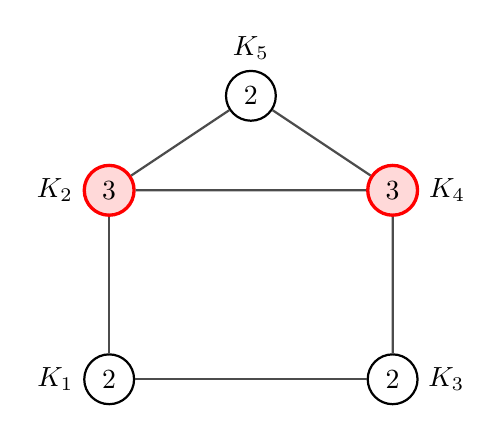
\begin{tikzpicture}[scale=1.2]
        \node[vertex, label=left:{$K_1$}] (K1) at (0, 0) {$2$};
        \node[oddvertex, label=left:{$K_2$}] (K2) at (0, 2) {$3$};
        \node[vertex, label=right:{$K_3$}] (K3) at (3, 0) {$2$};
        \node[oddvertex, label=right:{$K_4$}] (K4) at (3, 2) {$3$};
        \node[vertex, label=above:{$K_5$}] (K5) at (1.5, 3) {$2$};

        \draw[edge] (K1) -- (K2);
        \draw[edge] (K2) -- (K5);
        \draw[edge] (K5) -- (K4);
        \draw[edge] (K4) -- (K3);
        \draw[edge] (K1) -- (K3);
        \draw[edge] (K2) -- (K4);
    \end{tikzpicture}
    \caption{A mélygarázs úthálózata a kereszteződésekbe beírt fokszámokkal.}
    \label{fig:parking_graph}
\end{figure}

\textbf{3. Lépés:} Értékeljük az eredményt Euler tétele alapján:
\begin{itemize}
    \item Páratlan fokszámú csúcsok: $K_2$ (foka 3) és $K_4$ (foka 3). Ez összesen \textbf{pontosan 2 darab} páratlan csúcs.
    \item A többi csúcs ($K_1, K_3, K_5$) foka 2, tehát páros.
\end{itemize}

\textbf{Válasz:} Igen, a séta megvalósítható! Az őrnek csupán arra kell figyelnie, hogy a túrát a két páratlan csúcs valamelyikéből (tehát vagy a $K_2$, vagy a $K_4$ kereszteződésből) kell indítania, és a bejárás végén a másik páratlan kereszteződésbe fog megérkezni.
\end{example}

---

\section{Összefoglaló táblázat}

Mentésként készítettem neked egy gyors áttekintő táblázatot. Ezt tanuld meg, és nem érhet meglepetés!

\begin{table}[H]
    \centering
    \resizebox{\linewidth}{!}{%
    \begin{tabular}{lp{6.5cm}c}
        \toprule
        \textbf{Fogalom} & \textbf{Lényeg / Tulajdonság} & \textbf{Kulcsképlet} \\
        \midrule
        \textbf{Kézfogási lemma} & A fokszámok összege az élek számának kétszerese. & $\sum d(v) = 2|E|$ \\
        \textbf{Páratlan csúcsok} & Számuk minden egyszerű gráfban páros. & -- \\
        \textbf{Teljes gráf ($K_n$)} & Mindenki össze van kötve mindenkivel. & $|E| = \frac{n(n-1)}{2}$ \\
        \textbf{Fa gráf} & Összefüggő és körmentes gráf. & $|E| = n - 1$ \\
        \textbf{Komplementer gráf ($\bar{G}$)} & Ugyanazok a csúcsok, élek ott, ahol $G$-ben hiányoznak. & $|E| + |\bar{E}| = \binom{n}{2}$ \\
        \textbf{Izomorf gráfok} & Ugyanaz a struktúra, csak másképp rajzolva/címkézve. & -- \\
        \textbf{Zárt Euler-vonal} & Egy vonallal rajzolható, önmagába tér vissza. & Minden csúcs páros \\
        \textbf{Nyílt Euler-vonal} & Egy vonallal rajzolható más végponttal. & Pontosan 2 páratlan csúcs \\
        \bottomrule
    \end{tabular}%
    }
    \caption{A legfontosabb gráfos összefüggések egy helyen.}
    \label{tab:summary}
\end{table}

\end{document}